\documentclass[conference]{IEEEtran}

% *** CITATION PACKAGES ***
%
\usepackage{cite}
% cite.sty was written by Donald Arseneau
% V1.6 and later of IEEEtran pre-defines the format of the cite.sty package
% \cite{} output to follow that of IEEE. Loading the cite package will
% result in citation numbers being automatically sorted and properly
% "compressed/ranged". e.g., [1], [9], [2], [7], [5], [6] without using
% cite.sty will become [1], [2], [5]--[7], [9] using cite.sty. cite.sty's
% \cite will automatically add leading space, if needed. Use cite.sty's
% noadjust option (cite.sty V3.8 and later) if you want to turn this off.
% cite.sty is already installed on most LaTeX systems. Be sure and use
% version 4.0 (2003-05-27) and later if using hyperref.sty. cite.sty does
% not currently provide for hyperlinked citations.
% The latest version can be obtained at:
% http://www.ctan.org/tex-archive/macros/latex/contrib/cite/
% The documentation is contained in the cite.sty file itself.

% *** GRAPHICS RELATED PACKAGES ***
%
\ifCLASSINFOpdf
   \usepackage[pdftex]{graphicx}
  % declare the path(s) where your graphic files are
  % \graphicspath{{../pdf/}{../jpeg/}}
  % and their extensions so you won't have to specify these with
  % every instance of \includegraphics
  % \DeclareGraphicsExtensions{.pdf,.jpeg,.png}
\else
  % or other class option (dvipsone, dvipdf, if not using dvips). graphicx
  % will default to the driver specified in the system graphics.cfg if no
  % driver is specified.
  % \usepackage[dvips]{graphicx}
  % declare the path(s) where your graphic files are
  % \graphicspath{{../eps/}}
  % and their extensions so you won't have to specify these with
  % every instance of \includegraphics
  % \DeclareGraphicsExtensions{.eps}
\fi
% graphicx was written by David Carlisle and Sebastian Rahtz. It is
% required if you want graphics, photos, etc. graphicx.sty is already
% installed on most LaTeX systems. The latest version and documentation can
% be obtained at: 
% http://www.ctan.org/tex-archive/macros/latex/required/graphics/
% Another good source of documentation is "Using Imported Graphics in
% LaTeX2e" by Keith Reckdahl which can be found as epslatex.ps or
% epslatex.pdf at: http://www.ctan.org/tex-archive/info/
%
% latex, and pdflatex in dvi mode, support graphics in encapsulated
% postscript (.eps) format. pdflatex in pdf mode supports graphics
% in .pdf, .jpeg, .png and .mps (metapost) formats. Users should ensure
% that all non-photo figures use a vector format (.eps, .pdf, .mps) and
% not a bitmapped formats (.jpeg, .png). IEEE frowns on bitmapped formats
% which can result in "jaggedy"/blurry rendering of lines and letters as
% well as large increases in file sizes.
%
% You can find documentation about the pdfTeX application at:
% http://www.tug.org/applications/pdftex





% *** MATH PACKAGES ***
%
%\usepackage[cmex10]{amsmath}
% A popular package from the American Mathematical Society that provides
% many useful and powerful commands for dealing with mathematics. If using
% it, be sure to load this package with the cmex10 option to ensure that
% only type 1 fonts will utilized at all point sizes. Without this option,
% it is possible that some math symbols, particularly those within
% footnotes, will be rendered in bitmap form which will result in a
% document that can not be IEEE Xplore compliant!
%
% Also, note that the amsmath package sets \interdisplaylinepenalty to 10000
% thus preventing page breaks from occurring within multiline equations. Use:
%\interdisplaylinepenalty=2500
% after loading amsmath to restore such page breaks as IEEEtran.cls normally
% does. amsmath.sty is already installed on most LaTeX systems. The latest
% version and documentation can be obtained at:
% http://www.ctan.org/tex-archive/macros/latex/required/amslatex/math/





% *** SPECIALIZED LIST PACKAGES ***
%
%\usepackage{algorithmic}
% algorithmic.sty was written by Peter Williams and Rogerio Brito.
% This package provides an algorithmic environment fo describing algorithms.
% You can use the algorithmic environment in-text or within a figure
% environment to provide for a floating algorithm. Do NOT use the algorithm
% floating environment provided by algorithm.sty (by the same authors) or
% algorithm2e.sty (by Christophe Fiorio) as IEEE does not use dedicated
% algorithm float types and packages that provide these will not provide
% correct IEEE style captions. The latest version and documentation of
% algorithmic.sty can be obtained at:
% http://www.ctan.org/tex-archive/macros/latex/contrib/algorithms/
% There is also a support site at:
% http://algorithms.berlios.de/index.html
% Also of interest may be the (relatively newer and more customizable)
% algorithmicx.sty package by Szasz Janos:
% http://www.ctan.org/tex-archive/macros/latex/contrib/algorithmicx/




% *** ALIGNMENT PACKAGES ***
%
%\usepackage{array}
% Frank Mittelbach's and David Carlisle's array.sty patches and improves
% the standard LaTeX2e array and tabular environments to provide better
% appearance and additional user controls. As the default LaTeX2e table
% generation code is lacking to the point of almost being broken with
% respect to the quality of the end results, all users are strongly
% advised to use an enhanced (at the very least that provided by array.sty)
% set of table tools. array.sty is already installed on most systems. The
% latest version and documentation can be obtained at:
% http://www.ctan.org/tex-archive/macros/latex/required/tools/


%\usepackage{mdwmath}
%\usepackage{mdwtab}
% Also highly recommended is Mark Wooding's extremely powerful MDW tools,
% especially mdwmath.sty and mdwtab.sty which are used to format equations
% and tables, respectively. The MDWtools set is already installed on most
% LaTeX systems. The lastest version and documentation is available at:
% http://www.ctan.org/tex-archive/macros/latex/contrib/mdwtools/


% IEEEtran contains the IEEEeqnarray family of commands that can be used to
% generate multiline equations as well as matrices, tables, etc., of high
% quality.


%\usepackage{eqparbox}
% Also of notable interest is Scott Pakin's eqparbox package for creating
% (automatically sized) equal width boxes - aka "natural width parboxes".
% Available at:
% http://www.ctan.org/tex-archive/macros/latex/contrib/eqparbox/





% *** SUBFIGURE PACKAGES ***
%\usepackage[tight,footnotesize]{subfigure}
% subfigure.sty was written by Steven Douglas Cochran. This package makes it
% easy to put subfigures in your figures. e.g., "Figure 1a and 1b". For IEEE
% work, it is a good idea to load it with the tight package option to reduce
% the amount of white space around the subfigures. subfigure.sty is already
% installed on most LaTeX systems. The latest version and documentation can
% be obtained at:
% http://www.ctan.org/tex-archive/obsolete/macros/latex/contrib/subfigure/
% subfigure.sty has been superceeded by subfig.sty.



%\usepackage[caption=false]{caption}
%\usepackage[font=footnotesize]{subfig}
% subfig.sty, also written by Steven Douglas Cochran, is the modern
% replacement for subfigure.sty. However, subfig.sty requires and
% automatically loads Axel Sommerfeldt's caption.sty which will override
% IEEEtran.cls handling of captions and this will result in nonIEEE style
% figure/table captions. To prevent this problem, be sure and preload
% caption.sty with its "caption=false" package option. This is will preserve
% IEEEtran.cls handing of captions. Version 1.3 (2005/06/28) and later 
% (recommended due to many improvements over 1.2) of subfig.sty supports
% the caption=false option directly:
%\usepackage[caption=false,font=footnotesize]{subfig}
%
% The latest version and documentation can be obtained at:
% http://www.ctan.org/tex-archive/macros/latex/contrib/subfig/
% The latest version and documentation of caption.sty can be obtained at:
% http://www.ctan.org/tex-archive/macros/latex/contrib/caption/




% *** FLOAT PACKAGES ***
%
%\usepackage{fixltx2e}
% fixltx2e, the successor to the earlier fix2col.sty, was written by
% Frank Mittelbach and David Carlisle. This package corrects a few problems
% in the LaTeX2e kernel, the most notable of which is that in current
% LaTeX2e releases, the ordering of single and double column floats is not
% guaranteed to be preserved. Thus, an unpatched LaTeX2e can allow a
% single column figure to be placed prior to an earlier double column
% figure. The latest version and documentation can be found at:
% http://www.ctan.org/tex-archive/macros/latex/base/



%\usepackage{stfloats}
% stfloats.sty was written by Sigitas Tolusis. This package gives LaTeX2e
% the ability to do double column floats at the bottom of the page as well
% as the top. (e.g., "\begin{figure*}[!b]" is not normally possible in
% LaTeX2e). It also provides a command:
%\fnbelowfloat
% to enable the placement of footnotes below bottom floats (the standard
% LaTeX2e kernel puts them above bottom floats). This is an invasive package
% which rewrites many portions of the LaTeX2e float routines. It may not work
% with other packages that modify the LaTeX2e float routines. The latest
% version and documentation can be obtained at:
% http://www.ctan.org/tex-archive/macros/latex/contrib/sttools/
% Documentation is contained in the stfloats.sty comments as well as in the
% presfull.pdf file. Do not use the stfloats baselinefloat ability as IEEE
% does not allow \baselineskip to stretch. Authors submitting work to the
% IEEE should note that IEEE rarely uses double column equations and
% that authors should try to avoid such use. Do not be tempted to use the
% cuted.sty or midfloat.sty packages (also by Sigitas Tolusis) as IEEE does
% not format its papers in such ways.





% *** PDF, URL AND HYPERLINK PACKAGES ***
%
%\usepackage{url}
% url.sty was written by Donald Arseneau. It provides better support for
% handling and breaking URLs. url.sty is already installed on most LaTeX
% systems. The latest version can be obtained at:
% http://www.ctan.org/tex-archive/macros/latex/contrib/misc/
% Read the url.sty source comments for usage information. Basically,
% \url{my_url_here}.





% *** Do not adjust lengths that control margins, column widths, etc. ***
% *** Do not use packages that alter fonts (such as pslatex).         ***
% There should be no need to do such things with IEEEtran.cls V1.6 and later.
% (Unless specifically asked to do so by the journal or conference you plan
% to submit to, of course. )


% correct bad hyphenation here
\hyphenation{op-tical net-works semi-conduc-tor}

%% Key definitions for text elements. USE THEM
\def\secref#1{Sec.~\ref{#1}}
\def\figref#1{Fig.~\ref{#1}}
\def\tabref#1{Tab.~\ref{#1}}
\def\eqref#1{Eq.~(\ref{#1})}
\def\algref#1{Alg.~\ref{#1}}

\newcommand\etal{\emph{et al.}}

\usepackage{amsopn}


\newcommand{\bJidx}[1]{\ensuremath{\mathbf{J}^{[#1]}}}
\newcommand{\cose}{\mathrm{cose}}
\newcommand{\bzidx}[1]{\mathbf{z}^{[{#1}]}}
\newcommand{\bxidx}[1]{\mathbf{x}^{[{#1}]}}
\newcommand{\bhidx}[1]{\mathbf{h}^{[{#1}]}}
\newcommand{\bOmegaidx}[1]{\mathbf{\Omega}^{[{#1}]}}
\newcommand{\bSigmaidx}[1]{\mathbf{\Sigma}^{[{#1}]}}
\newcommand{\bHidx}[1]{\mathbf{H}^{[{#1}]}}

\newcommand{\bv}{\mathbf{v}}
\newcommand{\bl}{\mathbf{l}}
\newcommand{\bt}{\mathbf{t}}
\newcommand{\bo}{\mathbf{o}}
\newcommand{\bM}{\mathbf{M}}
\newcommand{\bL}{\mathbf{L}}
\newcommand{\bA}{\mathbf{A}}
\newcommand{\bB}{\mathbf{B}}
\newcommand{\bE}{\mathbf{E}}
\newcommand{\bK}{\mathbf{K}}
\newcommand{\bC}{\mathbf{C}}
\newcommand{\bG}{\mathbf{G}}
\newcommand{\bH}{\mathbf{H}}
\newcommand{\bI}{\mathbf{I}}
\newcommand{\bP}{\mathbf{P}}
\newcommand{\bX}{\mathbf{X}}
\newcommand{\bZ}{\mathbf{Z}}
\newcommand{\bR}{\mathbf{R}}
\newcommand{\bS}{\mathbf{S}}
\newcommand{\bU}{\mathbf{U}}
\newcommand{\bV}{\mathbf{V}}
\newcommand{\bT}{\mathbf{T}}
\newcommand{\bpi}{\mathbf{\pi}}
\newcommand{\btl}{\mathbf{tl}}
\newcommand{\bbr}{\mathbf{br}}


\newcommand{\iD}{\mathbf{D}}
\newcommand{\iN}{\mathbf{N}}
\newcommand{\iI}{\mathbf{I}}

\newcommand\norm[1]{\left\lVert#1\right\rVert}

\newcommand{\bzridx}[1]{\ensuremath{\mathbf{z}^{({#1})}}}
\newcommand{\bxridx}[1]{\mathbf{x}^{({#1})}}
\newcommand{\bhridx}[1]{\mathbf{h}^{({#1})}}

\newcommand{\bJ}{\mathbf{J}}
\newcommand{\bZero}{\mathbf{0}}

\newcommand{\cS}{\mathcal{S}}
\newcommand{\cG}{\mathcal{G}}
\newcommand{\cE}{\mathcal{E}}
\newcommand{\cC}{\mathcal{C}}
\newcommand{\cSM}{\mathcal{SM}}
\newcommand{\cR}{\mathcal{R}}
\newcommand{\cM}{\mathcal{M}}
\newcommand{\cP}{\mathcal{P}}
\newcommand{\cL}{\mathcal{L}}
\newcommand{\cD}{\mathcal{D}}
\newcommand{\cZ}{\mathcal{Z}}
\newcommand{\cX}{\mathcal{X}}
\newcommand{\range}[3]{#1_{#2:#3}}


\newcommand{\ba}{\mathbf{a}}
\newcommand{\bb}{\mathbf{b}}
\newcommand{\bc}{\mathbf{c}}
\newcommand{\bd}{\mathbf{d}}
\newcommand{\be}{\mathbf{e}}
\newcommand{\ec}{\mathbf{e}}
\newcommand{\bm}{\mathbf{m}}
\newcommand{\bg}{\mathbf{g}}
\newcommand{\Dim}{\mathrm{Dim}}

\newcommand{\bs}{\mathbf{s}}
\newcommand{\bx}{\mathbf{x}}
\newcommand{\by}{\mathbf{y}}
\newcommand{\br}{\mathbf{r}}
\newcommand{\bz}{\mathbf{z}}
\newcommand{\bu}{\mathbf{u}}
\newcommand{\bn}{\mathbf{n}}
\newcommand{\bh}{\mathbf{h}}
\newcommand{\bff}{\mathbf{f}}
\newcommand{\bp}{\mathbf{p}}
\newcommand{\bDelta}{\mathbf{\Delta}}
\newcommand{\bGamma}{\mathbf{\Gamma}}
\newcommand{\bDeltaalpha}{\mathbf{\Delta \alpha}}
\newcommand{\bDeltar}{\mathbf{\Delta r}}
\newcommand{\bDeltax}{\mathbf{\Delta x}}
\newcommand{\bDeltaX}{\mathbf{\Delta X}}
\newcommand{\bDeltat}{\mathbf{\Delta t}}
\newcommand{\bDeltaR}{\mathbf{\Delta R}}
\newcommand{\tTov}{\mathrm{t2v}}
\newcommand{\vTot}{\mathrm{v2t}}

\newcommand{\bO}{\mathbf{O}}

\newcommand{\defeq}{=}


\newcommand{\bmu}{\mathbf{\mu}}
\newcommand{\bnu}{\mathbf{\nu}}
\newcommand{\bSigma}{\mathbf{\Sigma}}
\newcommand{\bOmega}{\mathbf{\Omega}}
\newcommand{\bLambda}{\mathbf{\Lambda}}

\newcommand{\mat}[1]{#1}
\newcommand{\mbf}[1]{\mathbf{#1}}
\newcommand{\defn}[1]{\emph{#1}}

\newcommand{\mysum}{\sum}
\newcommand{\myprod}{\prod}
\newcommand{\eq}{=}
\newcommand{\pv}{\mathrm{P}}
%\newcommand{\implies}{\Rightarrow}
\newcommand{\Parents}{\mathrm{Parents}}
\newcommand{\rj}{\mathrm{j}}
\newcommand{\proj}{\mathrm{proj}}
\DeclareMathOperator*{\argmax}{argmax}
\DeclareMathOperator*{\argmin}{argmin}
\DeclareMathOperator*{\atantwo}{atantwo}

\newcommand{\mR}{\mathbb{R}}
\newcommand{\mN}{\mathbb{N}}
\newcommand{\mC}{\mathbb{C}}



\begin{document}
%
% paper title
% can use linebreaks \\ within to get better formatting as desired
\title{Active Semantic Mapping}


% author names and affiliations
% use a multiple column layout for up to three different
% affiliations
%\author{\IEEEauthorblockN{Federico Nardi} \and
%  \IEEEauthorblockN{Roberto Capobianco} \and \IEEEauthorblockN{Daniele
%    Nardi}}


% conference papers do not typically use \thanks and this command
% is locked out in conference mode. If really needed, such as for
% the acknowledgment of grants, issue a \IEEEoverridecommandlockouts
% after \documentclass

% for over three affiliations, or if they all won't fit within the width
% of the page, use this alternative format:
% 
\author{\IEEEauthorblockN{Federico Nardi\IEEEauthorrefmark{1}, Roberto
    Capobianco\IEEEauthorrefmark{1} and Daniele
    Nardi\IEEEauthorrefmark{1}}
  \IEEEauthorblockA{\IEEEauthorrefmark{1}Department of Computer,
    Control, and Management Engineering Antonio Ruberti\\ Sapienza
    University of Rome, Rome, Italy \\ Email:
    \{\textit{fnardi,capobianco,nardi}\}@diag.uniroma1.it}}

% make the title area
\maketitle

\begin{abstract}
%\boldmath
The abstract goes here.
\end{abstract}

% For peer review papers, you can put extra information on the cover
% page as needed:
% \ifCLASSOPTIONpeerreview
% \begin{center} \bfseries EDICS Category: 3-BBND \end{center}
% \fi
%
% For peerreview papers, this IEEEtran command inserts a page break and
% creates the second title. It will be ignored for other modes.
\IEEEpeerreviewmaketitle



\section{Introduction}

\subsubsection{Sometimes active perception is needed}
the last decade has seen tremendous advances in building accurate
digital models of the robot workspace. State-of-the-art reconstruction
and recognition approaches enable the robot to store precise geometric
and semantic information of objects/places in its internal
representation of the environment.

Still, some tasks require the robot to acquire a rich amount of
information about its workspace. As an example, for object
manipulation the robot needs to know the position of the objects in
the scene and their shape to plan a motion trajectory.

To represent this information a possible solution is to use CAD
models. While effective, this approach has the limitation that the
perceivable objects must be known a priori. To overcome this
limitation, one must provide the robot with the ability of actively
building such models to support task execution.

\subsubsection{Building a usable representation}
we are solving the problem of building a digital representation of the
robot workspace that can support task execution.

\subsubsection{enrich semantic mapping with active perception}
To this end, we enrich the robot software architecture with an active
vision module.

\subsubsection{active semantic mapping}
the active vision strategy takes as input the semantic map and returns
the NBV that increases the robot knowledge about a particular object.

\begin{figure}[t]
  \centering
 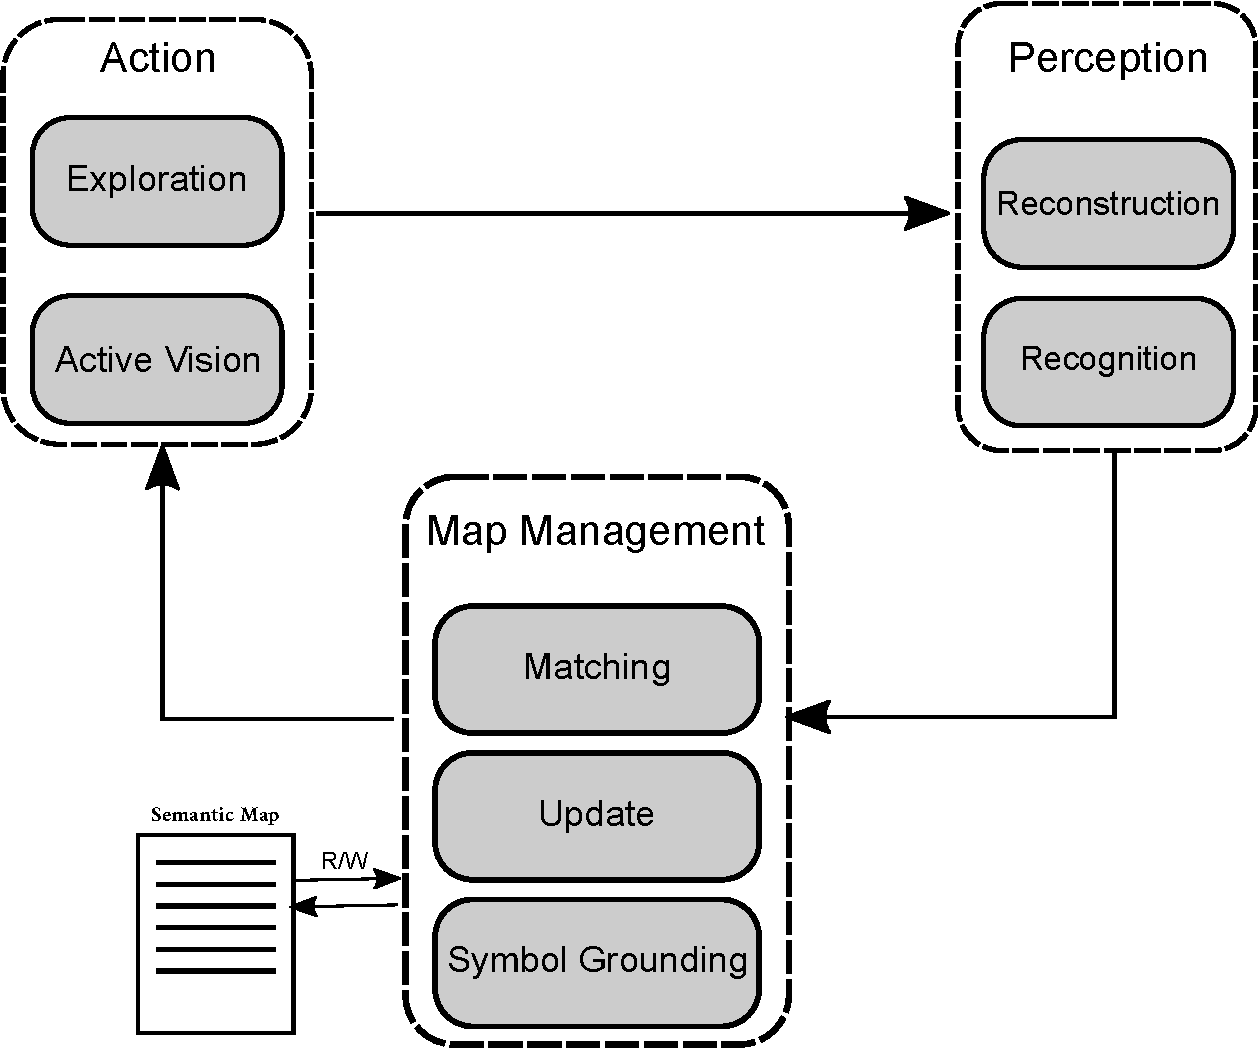
\includegraphics[width=\linewidth]{pics/motivation}
 \caption{Motivating Example. Provide a caption that lets the reader
   understand the image easily.  This image should be on top of the
   right column of page~1.}
  \label{fig:motivation}
\end{figure}
\section{Related Work}

\subsection{Reconstruction}

Consists in processing sensor measurements $\cS$ to recover both the
set of robot poses $\cX = \{ \bx_1 \dots \bx_T \}$ and a digital
representation of the environment $\cM$. In robotic applications, it
is mainly performed by addressing the "Simultaneous Localization and
Mapping" (SLAM) problem. The advent of affordable RGB-D sensors gave a
strong impulse in this investigation field and the proposed solutions
can be categorized according to how the scene surface is represented
\cite{cadena2016ieeetransrob}.

In the majority of SLAM methods, the scene is represented by a set of
sparse 3D landmarks that correspond to relevant features in the
environment (e.g. edges, corners) \cite{mur2015ieeetransrob}. These
methods are attractive because they're based on a lightweight
formulation and still they're effective in accurately localizing the
robot, but they provide a rather poor representation of the
environment since they tend to filter out portions with less features.

A different approach is to describe the 3D geometry by means of large
unstructured set of points (i.e., point clouds), which are obtained by
nowadays easily available RGB-D cameras. Contrary to landmark-based
methods, there are also "direct" methods that estimate the trajectory
of the robot and a 3D model directly from the intensity values and/or
depth values of all the image pixels
\cite{newcombe2011ICCV,steinbrucker2011real}. This type of
representation allows to better infer the structure of the scene but
it still may contain artifacts in some portions of the environment due
to the uneven sensor sampling density.

A reasonable choice to overcome this limitation is to introduce
structured representations, such as the ones used in Computer Graphics
for Surface Reconstruction \cite{berger2014state}. These are called
"boundary representations", since they define 3D objects in terms of
their surface boundary. In general, b-reps can be classified as:
curve-based representations (NURBS or B-Spline), mesh representations
(triangulated surfaces) and implicit representations (level-set
surfaces). The latter was investigated in the work of Newcombe et
al. \cite{newcombe2011kinectfusion} and received much interest from
the SLAM community thanks to its representation power. The main
drawback is the not negligible amount of memory required also in the
case of small scale scenes. This limits considerably the scalability
of this method and the development of optimized techniques for
large-scale environments is an open issue
\cite{kahler2015very,vespa2018efficient}.

All the representations mentioned so far describe the environment
surface by means of low-level features. Another approach, proposed in
the seminal work by Moreno~\etal \cite{salas2013CVPR}, is to
investigate higher level object-based representations, where the map
is made of objects and solid shapes as it is the case in Computer
Aided Design (CAD).

\subsection{Recognition}

Consists in extracting subsets of sensory data (patterns) belonging to
known objects and scenes categories and assign them the corresponding
semantic label. Typically, in robotic applications input data can be
of two types: \emph{raw}, recognition is performed directly on sensor
data and each time the sensor returns a measurement;
\emph{reconstructed}, recognition is performed on a scene obtained
with reconstruction methods. The output of the recognition step
consists in a list of detections $\cD = \{ \bd_1 \dots \bd_N \}$,
that, in general, may contain just one element (classification) or a
sequence of them (detection, segmentation). Each entry in the
detection list $\bd_i$ is characterized by:
\begin{itemize}
	\item {\bf Semantic Label}: that identifies the semantic category of the detection. 
	\item {\bf Spatial Location}: that express the position of the detection w.r.t. the reference system of the input data.
\end{itemize}

Recognition can be decomposed into sub-tasks, depending on the
information one is interested to extract from the input data. These
sub-tasks can be organized on a progression that goes from coarse to
fine grained inference.

Image classification is the task of assigning a semantic label to an
input image from a fixed set of categories. Ulrich and Nourbakhsh
\cite{ulrich2000icra} propose an appearance-based place recognition
system for topological localization. They use colour histogram
features \cite{swain1991ijcv} and a simple voting scheme for
nearest-neighbor matching. In a similar fashion, Torralba
\etal~\cite{torralba2003context} derive an hidden Markov model (HMM)
for place recognition and new place categorisation based on the global
statistic feature retrieved from texture \cite{oliva2001ijcv}. In
contrast, Lisin \etal~\cite{lisin2005cvpr} propose to model classes of
images as a probability distribution over local features, in order to
be combined with global features. This method has proven to perform
well in applications where a rough segmentation of objects is
available.

Object detection consists of making a prediction not only of object
categories but also of their spatial locations. A seminal work can be
considered that of Viola and Jones \cite{viola2004ijcv}, who proposed
a fast and robust face detection. Their method makes use of Haar-like
features \cite{papageorgiou1998iccv} to search for likely face
candidates, which can then be refined using a cascade of more
expensive but selective detection algorithms
\cite{freund1997jcss}. Likewise, a well-known example of pedestrian
detection has been proposed by Dalal and Triggs \cite{dalal2005cvpr},
who use a set of overlapping Histogram of Oriented Gradients (HOG)
descriptors fed into a Support Vector Machine (SVM)
\cite{cortes1995support}.

Image segmentation is the task of finding groups of pixels that
possess some "similarity" and is one of the oldest and most widely
studied problems in computer vision.  Early techniques focus on local
region merging and splitting
\cite{ohlander1978picture,brice1970scene}, while, more recent
algorithms often optimize some global criterion, such as intra-region
consistency and inter-region boundary lengths or dissimilarity
\cite{comaniciu2002pami,shi2000pami,felzenszwalb2004ijcv,chan2001ip,osher1988jcp}.

Despite the popularity of the presented methods, a recent breakthrough
in scene understanding has been the adoption of Convolutional Neural
Networks (CNNs) \cite{garcia2017review}. Krizhevsky \etal in
\cite{krizhevsky2012nipsjournal} present the pioneering deep CNN that,
despite its simplicity, won the Imagenet 2012 classification challenge
with wide margin on the closest competitor. Similarly, different
object detection methods based on deep neural netowrks have shown to
outperform the state-of-the-art
\cite{redmon2016cvpr,erhan2014cvpr,liu2016eccv}. Consequently, the
capabilities of such networks have been also investigated in
pixel-level labeling problems like semantic segmentation. In this
context, a milestone is the work of Long \etal~\cite{long2015cvpr} who
transformed existing classification models
(\cite{simonyan2014very,szegedy2015cvpr}) into fully convolutional
ones to output spatial maps instead of classification scores. One of
the main reason behind its popularity is that, with this approach,
CNNs can be trained end-to-end and efficiently learn to make dense
predictions with inputs of arbitrary size.

\section{System Overview}

In order to autonomously operate in human environments, robots need
the ability to build and maintain an internal representation of their
workspace. Traditional mapping techniques return a geometric model of
the environment that can be used for computing distances to obstacles
or finding paths toward goals. However, some manipulation and
navigation tasks may require human level knowledge (e.g.,
objects/places categories, functions, properties, and so on) to be
effectively executed, thus, requiring also the acquisition and
modeling of semantic information.

The problem of building such a representation of the environment can
be addressed by facing three aspects: 1) processing sensor data to
extract geometric and semantic information, 2) modeling these
information in a suitable representation that support task execution
and 3) planning the robot motion to maximize the extraction of such
information. In the past, these aspects have been separately addressed
by researchers who mainly focused on one of them assuming others were
already solved or not relevant.

In this work, we propose a general and complete semantic mapping
system that simultaneously aims at addressing in a unified framework
the three above mentioned sub-problems. This allows our system to be
effectively deployed in different scenarios, making a step towards the
next generation robotic applications.


\section{Conclusion}
The conclusion goes here.

% trigger a \newpage just before the given reference
% number - used to balance the columns on the last page
% adjust value as needed - may need to be readjusted if
% the document is modified later
%\IEEEtriggeratref{8}
% The "triggered" command can be changed if desired:
%\IEEEtriggercmd{\enlargethispage{-5in}}

% references section

% can use a bibliography generated by BibTeX as a .bbl file
% BibTeX documentation can be easily obtained at:
% http://www.ctan.org/tex-archive/biblio/bibtex/contrib/doc/
% The IEEEtran BibTeX style support page is at:
% http://www.michaelshell.org/tex/ieeetran/bibtex/
%\bibliographystyle{IEEEtran}
% argument is your BibTeX string definitions and bibliography database(s)
%\bibliography{IEEEabrv,../bib/paper}
%
% <OR> manually copy in the resultant .bbl file
% set second argument of \begin to the number of references
% (used to reserve space for the reference number labels box)


\bibliographystyle{ieeetr}
\bibliography{glorified,robots}



% that's all folks
\end{document}


